\section{Motivation}
\begin{frame}{Can reinforcement learning solve robotics?}
\begin{columns}[T]
\begin{column}{0.55\textwidth}
\footnotesize
\textbf{Alpha Go Zero}~\raisebox{-0.3em}{
\includegraphics[height=1.1em]{images/ddpg/figures/alpha-go-logo.jpg}}~(Silver et al, Nature, 2017)
\vspace{0.2em}

\scriptsize selecting among possible moves for that piece. We represent the policy $\pi(a|s)$ by a $8 \times 8 \times 73$ stack of planes encoding a probability distribution over \fbox{4{,}672 possible moves}. Each of the $8 \times 8$ positions identifies the square from which to ``pick up'' a piece. The first 56 planes encode\ldots

\vspace{0.6em}
\footnotesize
\textbf{Dota 5}~\raisebox{-0.3em}{
\includegraphics[height=1.1em]{images/ddpg/figures/dota-logo.jpg}}~(OpenAI et al, 2019, \href{https://cdn.openai.com/dota-2.pdf}{\scriptsize cdn.openai.com/dota-2.pdf})
\vspace{0.2em}

\scriptsize floats and categorical values with hundreds of possibilities) each time step. \fbox{We discretize the} action space; on an average timestep our model chooses among \fbox{8{,}000} to 80{,}000 actions (depending on hero). For comparison Chess requires around one thousand\ldots

\vspace{0.6em}
\footnotesize
\textbf{Alpha Star}~\raisebox{-0.3em}{
\includegraphics[height=1.1em]{images/ddpg/figures/alpha-go-logo.jpg}}~(Vinyals et al, Nature, 2019)
\vspace{0.2em}

\scriptsize observe and act next (Fig.~1a). This representation of actions in approximately \fbox{$10^{26}$ possible choices} at each step. Similar\ldots
\end{column}
\begin{column}{0.42\textwidth}
\begin{figure}
    \centering
    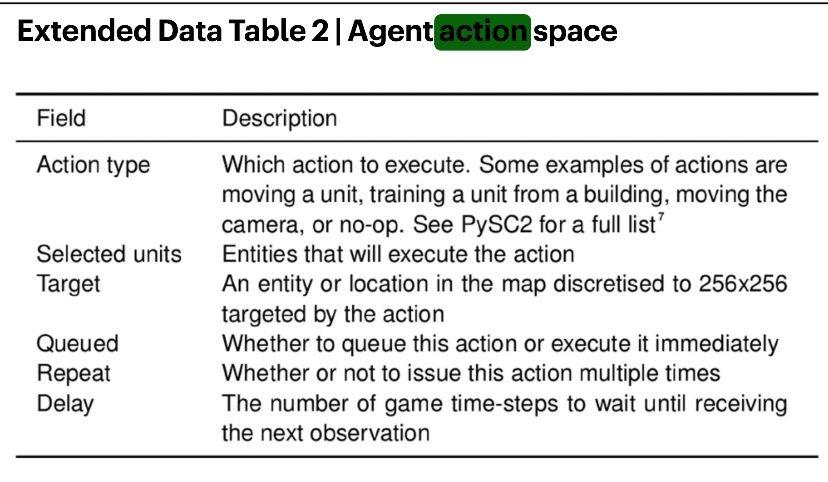
\includegraphics[width=\linewidth,height=0.85\textheight,keepaspectratio]{images/ddpg/figures/alpha-star.jpg}
\end{figure}
\end{column}
\end{columns}
\end{frame}

\begin{frame}{DDPG (Lillicrap et al, 2015)}
\vspace{2em}
\Large A first ``Deep'' crack at RL with continuous action spaces
\end{frame}
